\chapter{Die Faltung}
In diesem Kapitel wird erläutert, wie die Faltung (engl. \textit{convolution}) bei CNNs zu verstehen ist und wie diese Operation bei diesen neuronalen Netzen motiviert wird. In diesem Zusammenhang werden Begriffe wie Merkmalskarten (engl. \textit{feature maps}) und Filter (engl. \textit{kernels}) eingeführt. Des Weiteren wird die Arithmetik der Faltungsoperation für zweidimensionale Eingaben, repräsentiert durch Matrizen, erklärt und das Verfahren \textit{padding} beziehungsweise das Nutzen von \textit{strides} erläutert. Das gesamte Kapitel wird mit konkreten Beispielen begleitet, um die verschiedenen Effekte der Faltungsoperation zu beleuchten.

\section{Die Faltungsoperation}
In der Analysis ist die Faltung ein mathematischer Operator und liefert für zwei Funktionen $f$ und $g$ die Funktion $ f \ast g$, wobei mit dem Sternchen die Faltungsoperation gemeint ist.

\begin{defi}[Faltung]\label{allg_faltung}
    Für zwei Funktionen $f,g: \RRn \rightarrow \mathbb{C}$ ist die Faltung als
    \begin{equation*}
        (f \ast g) (x) := \int_{\RRn} f(\tau) g(x-\tau) \mathrm{d} \tau
    \end{equation*}
    definiert, wobei gefordert wird, dass das Integral für fast alle $x$ wohldefiniert ist.
   \end{defi}

Bei klassischen neuronalen Netzen, siehe Kapitel \ref{classicNN} werden Eingabedaten durch eine Verkettung von affinen Transformationen verarbeitet. Typischerweise wird die Eingabe als Vektor dargestellt und  mit einer Matrix multipliziert, gegebenenfalls mit einem Biasvektor manipuliert und schließlich so die Ausgabe generiert. Bilder-, Audio- oder Videoaufnahmen besitzen jedoch mehrere Merkmale in unterschiedlichen Achsen. Oft sind solche Eingabedaten im Bereich des Machine-Learnings als mehrdimensionale Arrays abgelegt, welche eine oder mehrere Achsen repräsentieren, wobei die Ordnung dieser eine Rolle spielt. Bei digitalisierten Bildern sind das bespielsweise die Höhe und Breite des Bildes, bei Audioaufnahmen gibt es nur eine Achse, und zwar die Zeitachse. Hinzu kommen Kanalachsen als weitere Verfeinerung der Daten, zum Beispiel besitzen RGB-Farbbilder drei Kanäle der Farben rot, grün und blau. 

Diese speziellen Eigenschaften können bei affinen Transformationen nicht berücksichtigt werden. Alle Merkmale sowie Achsen werden gewissermaßen gleich behandelt und die wesentliche topologische Struktur kann so nicht zum Vorteil ausgenutzt werden. Hier soll nun die sogenannte diskrete Faltung Abhilfe schaffen.

\begin{defi}[Diskrete Faltung]\label{disk_faltung}
    Für zwei Funktionen $f,g: D \rightarrow \mathbb{C}$ mit einem diskreten Definitionsbereich $D \subseteq \mathbb{Z}^n$ ist die diskrete Faltung als
    \begin{equation*}
        (f \ast g) (n) := \sum_{k \in D} f(k) g(x-k)
    \end{equation*}
    definiert. Hier wird über dem gesamten Definitionsbereich $D$ summiert. Ist $D$ beschränkt, werden $f$ beziehungsweise $g$ durch Nullen fortgesetzt. 
   \end{defi}

Besonders bei der Bildverarbeitung wird oft die diskrete Faltung als lineare Operation verwendet. 

\begin{defi}[Matrixfaltung, vgl. \cite{gruening}] \label{matrix_faltung}
    Für gegebene Matrizen $X \in \RR^{h \times w}$ und $K \in \RR^{k_h \times k_w}$ seien 
    \begin{equation*}
        h_l=\begin{cases}
           \lfloor k_h/2  \rfloor &, k_h \, \text{ungerade} \\
           k_h/2-1 &, \text{sonst}
        \end{cases}, \; \; 
        w_l=\begin{cases}
            \lfloor k_w/2 \rfloor &, k_w \, \text{ungerade} \\
            k_w/2 -1 &, \text{sonst}    
        \end{cases}.
    \end{equation*} 
    Die Matrixfaltung $K \ast X \in \RR^{h \times w}$ ist als 
    \begin{equation}
        \label{matrix_faltung_op}
        (K \ast X)_{i,j}:=\sum_{l=-h_l}^{\lfloor k_h/2  \rfloor} \sum_{m=-w_l}^{\lfloor k_w/2 \rfloor} K_{l+h_l+1, m+w_l+1} X_{i+l,j+m} \; \; \forall i \in [h], j \in [w]
    \end{equation} mit $X_{i,j}=0$ für $i \notin [h]$ und $j \notin [w]$ definiert.
    \end{defi}

\begin{bem}\label{bem_strides}
    Die Matrixfaltung kann durch viele weitere Parameter genauer spezifiziert werden. Sogannte \textit{strides} bestimmen die Reduktion bei der Faltung von $X$ in der Höhe $h$ beziehungsweise Breite $w$. Für strides $s_h, s_w \in \mathbb{N}$ ist die Matrixfaltung als
    \begin{equation*}
        (K \ast X)_{i,j}:=\sum_{l=-h_l}^{\lfloor k_h/2  \rfloor} \sum_{m=-w_l}^{\lfloor k_w/2 \rfloor} K_{l+h_l+1, m+w_l+1} X_{i \cdot s_h +l,j \cdot s_w +m} \; \; \forall i \in [h], j \in [w].
    \end{equation*}
    Für $s_h=s_w=1$ ergibt sich die Standardvariante wie in \ref{matrix_faltung_op}.
    \end{bem}

Im Folgenden werden konkrete Beispiele für verschiedene zweidimensionale Faltungen, welche in dieser Arbeit im Fokus stehen, gegeben. Dabei sind die Eingabe $X \in \RR^{h \times w}$ und der Filter $K \in \RR^{k_h \times k_w}$ immer als Matrizen zu verstehen. Das Ergebnis der Faltung $S= X \ast K$ wird als Merkmalskarte bezeichnet. Es sei angemerkt, dass oft $k_h=k_w$ sowie $k_h$ ungerade gewählt wird, z.B. $k_h=3$ oder $k_h=5$. Die Größe der Merkmalskarte wird durch die Parameter
\begin{itemize}
    \item $h,w$: Die Höhe und Breite der Eingabe,
    \item $k_h, k_w$: Die Abmessungen des Filters,
    \item $s_h, s_w$: Die Wahl der strides, 
    \item $p_h, p_w$: Die Größe des zero paddings
\end{itemize}
beeinflusst. Mit zero padding ist gemeint, dass künstliche Nullen um Randpixel der Eingabe $X$ eingefügt werden, damit die Berechnung mit dem Filter um jene Pixel gelingt. Ein Beispiel für das Verwenden von zero padding wird in Abbildung \ref{abb_simplematrixconv_padding} gezeigt. In Abbildung \ref{abb_simplematrixconv} ist die Berechnung einer einfachen zweidimensionalen Matrixfaltung dargestellt. Ein vorher festgelegter Filter (grau) bewegt sich über die Eingabe (blau) und berechnet jeweils die Einträge der Ausgabe(grün). 

\begin{figure}[h]
    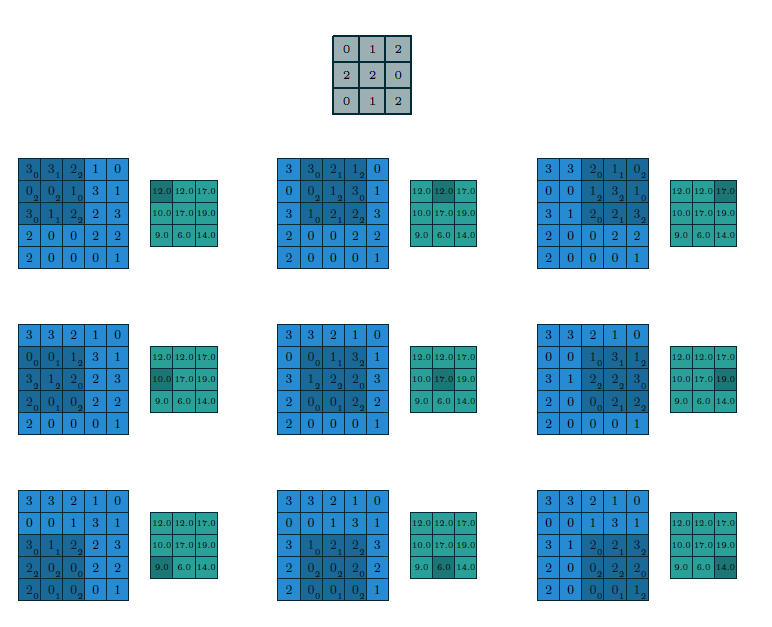
\includegraphics[width=0.8\textwidth]{pics/abb_simpleconv}
    \centering
    \caption{Es wird die Merkmalskarte $S \in \RR^{3 \times 3}$ mit den Parametern ${h,w=5}, k_h=k_w=3, s_h=s_w=1$ und $p_h=p_w=1.$}
    \label{abb_simplematrixconv}
\end{figure}

\begin{figure}[h]
    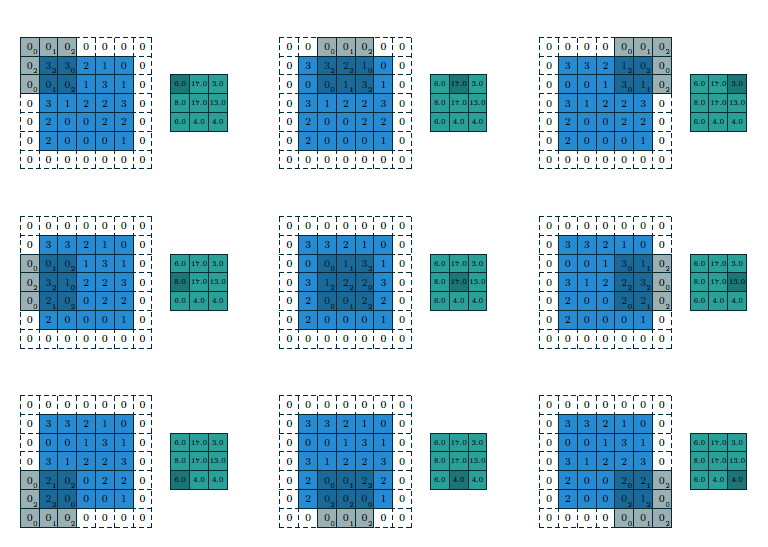
\includegraphics[width=0.8\textwidth]{pics/abb_simplecov_padding}
    \centering
    \caption{Es wird die Merkmalskarte $S \in \RR^{3 \times 3}$ mit den Parametern ${h,w=5}, k_h=k_w=3, s_h=s_w=2$ und $p_h=p_w=1$ berechnet.}
    \label{abb_simplematrixconv_padding}
\end{figure}



\section{Motivation der Faltung}
..
Sie nutzt wichtige Konzepte zur Optimierung von Machine-Learning-Verfahren wie spärliche Konnektivität (engl. \textit{sparse connectivity}), \textit{Parameter Sharing} und \textit{äquivariante Repräsentation}, vgl. \cite{goodfellow}. Spärlicher Konnektivität bedeutet, dass die Ausgabeeinheit auf einer bestimmten Schicht nur durch wenige Eingabeeinheiten beeinflusst wird. Dies ist bei CNNs typisch, da meist die verwendeten Filter viel kleiner als die Eingabe ist. Noch mehr erklären + Abbildung

Mit Parameter Sharing ist die Nutzung von gleichen Parametern für mehrere Funktionen im neuronalen Netz gemeint. In herkömmlichen Feed-Forward-Netzen wird jedes Element der Gewichtsmatrizen für die Berechnung der Aktivierungen der jeweiligen Schichten verwendet. Anschließend werden diese Gewichte dann nicht mehr gebraucht. Im Zusammenhang von CNNs bedeutet Parameter Sharing während der Faltungsoperation, dass nur eine bestimmte Menge von Parametern erlernt werden müssen
Noch mehr erklären + Abbildung

